\section{What's wrong with monocular camera?}
\label{mono_prob}

As the name suggests a monocular camera is a camera with a single imaging sensor. In section X. we say that given a perfectly calibrated camera ie. with the intrinsic and extrinsic parameters known, we can measure size of objects in the real world. This however is not true for a single image taken from a monocular camera. When 3D objects are projected onto the image plane (2D), the depth information stored in the z-axis is lost. This can be seen in the example below. 

% For one-column wide figures use
\begin{figure}
% Use the relevant command to insert your figure file.
% For example, with the graphicx package use
  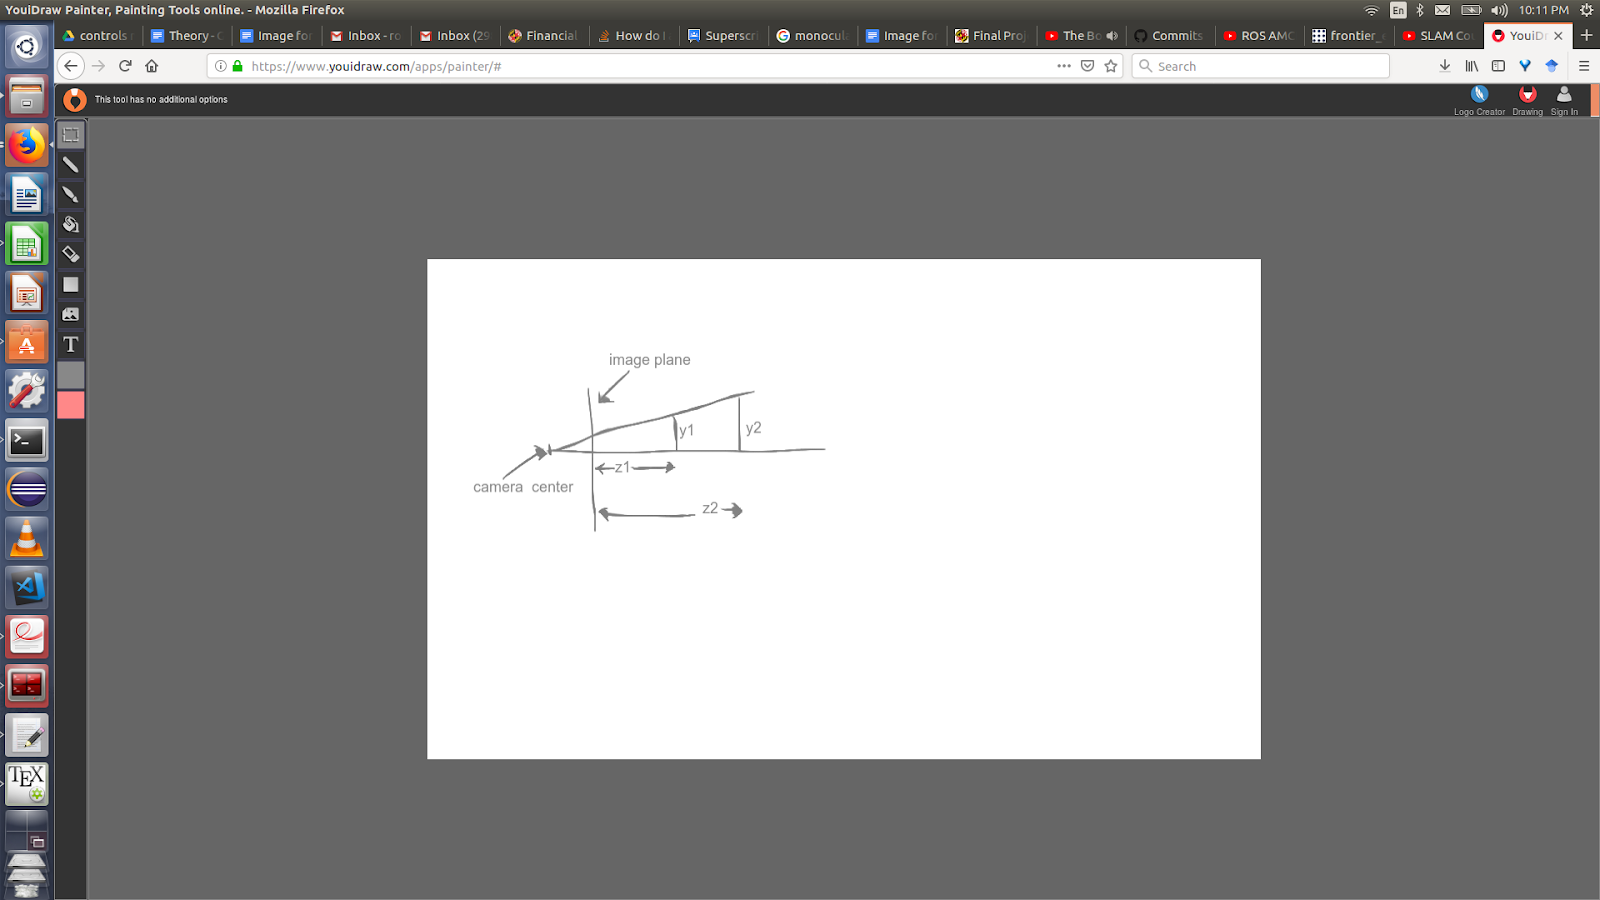
\includegraphics[width=\textwidth]{./figures/1.png}
% figure caption is below the figure
\caption{Monocular camera scale problem}
\label{fig:mono1}       % Give a unique label
\end{figure}

As seen in the Fig~\ref{fig:mono1}, irrespective of the location of the object in the real world, the size of the object in the image plane remains the same. Mathematically, this can be shown as 

\begin{equation}
\frac{y}{f}=\frac{y_1}{z_1+f}=\frac{y_2}{z_2+f}
\end{equation}

Where $f$ is the focal length of the camera. The title of the paper mentions scale estimation. In the context of SLAM which will be covered in the next section, scale is a term used to denote the factor by which the computed trajectory by a SLAM algorithm needs to be multiplied/scaled to make it equal to the ground truth. For example, if the measured distance is 2m, whereas the ground truth is 4m, the scale value would be 2. This is an area of active research and the community has come up with different techniques to solve this problem. As the title suggests, we would be talking about the fusion of IMU and Vision for solving this challenge.
